% Options for packages loaded elsewhere
\PassOptionsToPackage{unicode}{hyperref}
\PassOptionsToPackage{hyphens}{url}
%
\documentclass[
]{article}
\usepackage{lmodern}
\usepackage{amssymb,amsmath}
\usepackage{ifxetex,ifluatex}
\ifnum 0\ifxetex 1\fi\ifluatex 1\fi=0 % if pdftex
  \usepackage[T1]{fontenc}
  \usepackage[utf8]{inputenc}
  \usepackage{textcomp} % provide euro and other symbols
\else % if luatex or xetex
  \usepackage{unicode-math}
  \defaultfontfeatures{Scale=MatchLowercase}
  \defaultfontfeatures[\rmfamily]{Ligatures=TeX,Scale=1}
\fi
% Use upquote if available, for straight quotes in verbatim environments
\IfFileExists{upquote.sty}{\usepackage{upquote}}{}
\IfFileExists{microtype.sty}{% use microtype if available
  \usepackage[]{microtype}
  \UseMicrotypeSet[protrusion]{basicmath} % disable protrusion for tt fonts
}{}
\makeatletter
\@ifundefined{KOMAClassName}{% if non-KOMA class
  \IfFileExists{parskip.sty}{%
    \usepackage{parskip}
  }{% else
    \setlength{\parindent}{0pt}
    \setlength{\parskip}{6pt plus 2pt minus 1pt}}
}{% if KOMA class
  \KOMAoptions{parskip=half}}
\makeatother
\usepackage{xcolor}
\IfFileExists{xurl.sty}{\usepackage{xurl}}{} % add URL line breaks if available
\IfFileExists{bookmark.sty}{\usepackage{bookmark}}{\usepackage{hyperref}}
\hypersetup{
  pdftitle={DS 621 Fall2020: Homework 1 (Group3)},
  pdfauthor={Zach Alexander, Sam Bellows, Donny Lofland, Joshua Registe, Neil Shah, Aaron Zalki},
  hidelinks,
  pdfcreator={LaTeX via pandoc}}
\urlstyle{same} % disable monospaced font for URLs
\usepackage[margin=1in]{geometry}
\usepackage{graphicx,grffile}
\makeatletter
\def\maxwidth{\ifdim\Gin@nat@width>\linewidth\linewidth\else\Gin@nat@width\fi}
\def\maxheight{\ifdim\Gin@nat@height>\textheight\textheight\else\Gin@nat@height\fi}
\makeatother
% Scale images if necessary, so that they will not overflow the page
% margins by default, and it is still possible to overwrite the defaults
% using explicit options in \includegraphics[width, height, ...]{}
\setkeys{Gin}{width=\maxwidth,height=\maxheight,keepaspectratio}
% Set default figure placement to htbp
\makeatletter
\def\fps@figure{htbp}
\makeatother
\setlength{\emergencystretch}{3em} % prevent overfull lines
\providecommand{\tightlist}{%
  \setlength{\itemsep}{0pt}\setlength{\parskip}{0pt}}
\setcounter{secnumdepth}{-\maxdimen} % remove section numbering
\usepackage{geometry}
\usepackage{multicol}
\usepackage{multirow}
\usepackage{xcolor}
\usepackage{booktabs}
\usepackage{longtable}
\usepackage{array}
\usepackage{wrapfig}
\usepackage{float}
\usepackage{colortbl}
\usepackage{pdflscape}
\usepackage{tabu}
\usepackage{threeparttable}
\usepackage{threeparttablex}
\usepackage[normalem]{ulem}
\usepackage{makecell}

\title{DS 621 Fall2020: Homework 1 (Group3)}
\usepackage{etoolbox}
\makeatletter
\providecommand{\subtitle}[1]{% add subtitle to \maketitle
  \apptocmd{\@title}{\par {\large #1 \par}}{}{}
}
\makeatother
\subtitle{Moneyball Linear Regression}
\author{Zach Alexander, Sam Bellows, Donny Lofland, Joshua Registe, Neil Shah,
Aaron Zalki}
\date{}

\begin{document}
\maketitle

Source code:
\url{https://github.com/djlofland/DS621_F2020_Group3/tree/master/Homework_1}

\hypertarget{overview}{%
\subsection{Overview}\label{overview}}

In professional sports, there is a huge interest in attempting to
leverage historic statistics to both predict future outcomes
(wins/losses) and explore opportunities for tuning or improving a team
or individual's performance. This data-driven approach to sports has
gained a large following over the last decade and entered mass media in
the form of fantasy leagues, movies (e.g.~Moneyball), and
websites/podcasts (e.g.~FiveThirtyEight). In this analysis, we will be
using a classic baseball data set with the goal of building several
different models capable of predicting team wins over a season given
other team stats during that season (i.e.~homeruns, strikeouts, base
hits, etc).

We will first explore the data looking for issues or challenges
(i.e.~missing data, outliers, possible coding errors,
multicollinearlity, etc). Once we have a handle on the data, we will
apply any necessary cleaning steps. Once we have a reasonable dataset to
work with, we will build and evaluate three different linear models that
predict seasonal wins. Our dataset includes both training data and
evaluation data - we will train using the main training data, then
evaluate models based on how well they perform against the holdout
evaluation data. Finally we will select a final model that offers the
best compromise between accuracy and simplicity.

\hypertarget{data-exploration}{%
\subsection{1. Data Exploration}\label{data-exploration}}

\emph{Describe the size and the variables in the moneyball training data
set. Consider that too much detail will cause a manager to lose interest
while too little detail will make the manager consider that you aren't
doing your job. Some suggestions are given below. Please do NOT treat
this as a check list of things to do to complete the assignment. You
should have your own thoughts on what to tell the boss. These are just
ideas.}

\hypertarget{dataset}{%
\subsubsection{Dataset}\label{dataset}}

The moneyball training set contains 17 columns - including the target
variable ``TARGET\_WINS'' - and 2276 rows, covering baseball team
performance statistics from the years 1871 to 2006 inclusive. The data
has been adjusted to match the performance of a typical 162 game season.
The data-set was entirely numerical and contained no categorical
variables.

Below, we created a chart that describes each variable in the dataset
and the theoretical effect it will have on the number of wins projected
for a team.

\begin{figure}
\centering
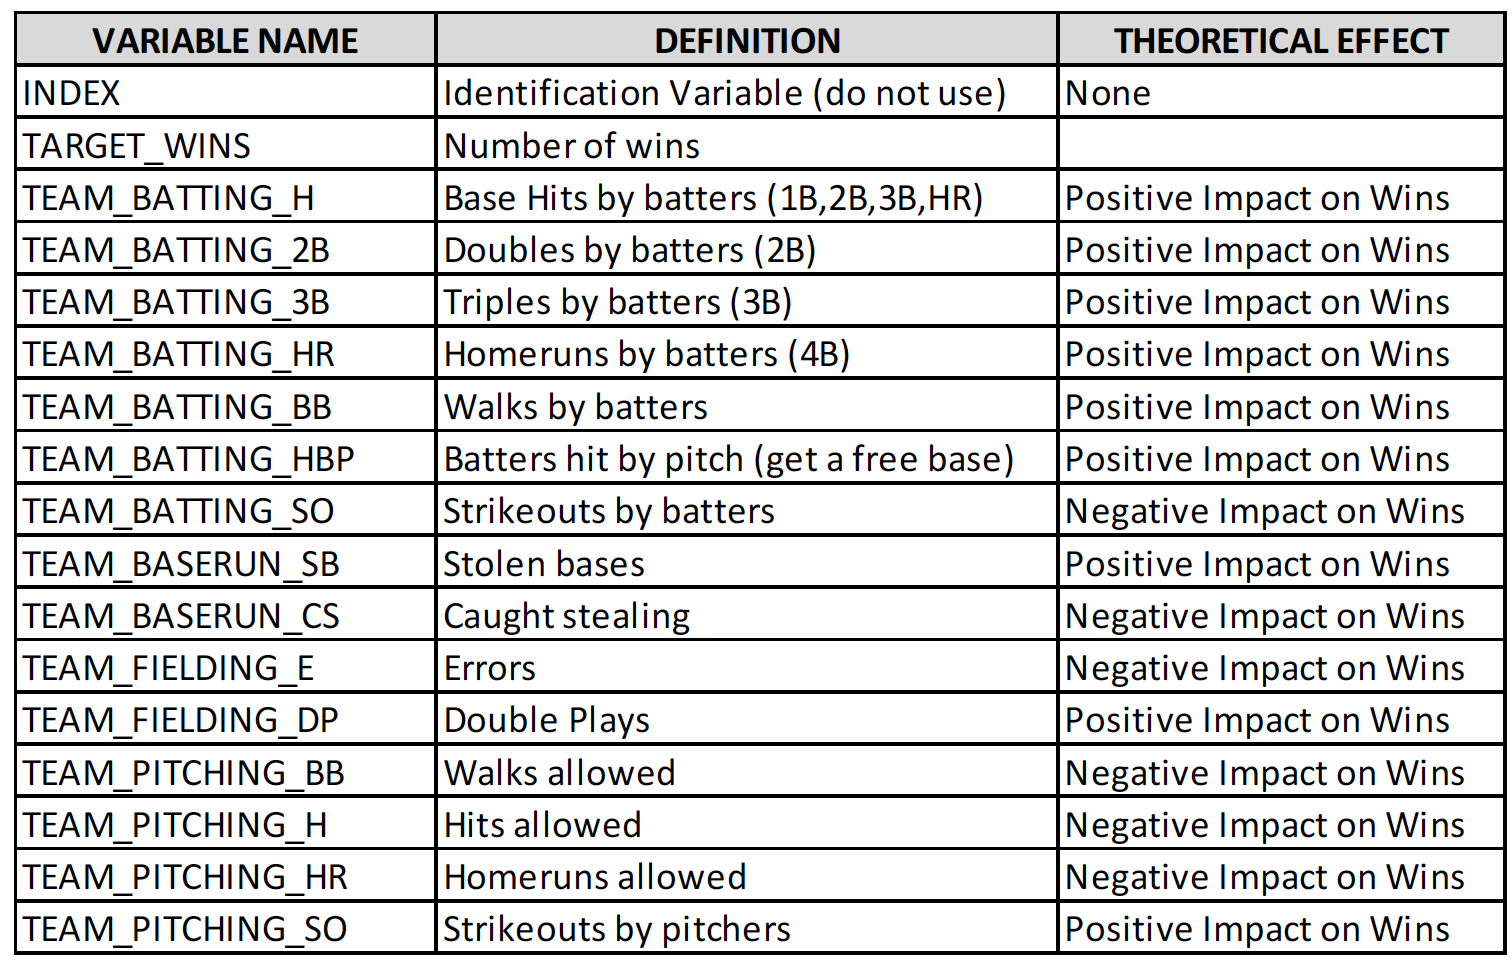
\includegraphics{./figures/Variables.png}
\caption{Variables of Interest}
\end{figure}

Given that the Index column had no impact on the target variable, number
of wins, it was dropped.

\hypertarget{summary-stats}{%
\subsubsection{Summary Stats}\label{summary-stats}}

We compiled summary statistics on our data set to better understand the
data before modeling.

\begin{verbatim}
##   TARGET_WINS       BATTING_H      BATTING_2B      BATTING_3B    
##  Min.   :  0.00   Min.   : 891   Min.   : 69.0   Min.   :  0.00  
##  1st Qu.: 71.00   1st Qu.:1383   1st Qu.:208.0   1st Qu.: 34.00  
##  Median : 82.00   Median :1454   Median :238.0   Median : 47.00  
##  Mean   : 80.79   Mean   :1469   Mean   :241.2   Mean   : 55.25  
##  3rd Qu.: 92.00   3rd Qu.:1537   3rd Qu.:273.0   3rd Qu.: 72.00  
##  Max.   :146.00   Max.   :2554   Max.   :458.0   Max.   :223.00  
##                                                                  
##    BATTING_HR       BATTING_BB      BATTING_SO       BASERUN_SB   
##  Min.   :  0.00   Min.   :  0.0   Min.   :   0.0   Min.   :  0.0  
##  1st Qu.: 42.00   1st Qu.:451.0   1st Qu.: 548.0   1st Qu.: 66.0  
##  Median :102.00   Median :512.0   Median : 750.0   Median :101.0  
##  Mean   : 99.61   Mean   :501.6   Mean   : 735.6   Mean   :124.8  
##  3rd Qu.:147.00   3rd Qu.:580.0   3rd Qu.: 930.0   3rd Qu.:156.0  
##  Max.   :264.00   Max.   :878.0   Max.   :1399.0   Max.   :697.0  
##                                   NA's   :102      NA's   :131    
##    BASERUN_CS     BATTING_HBP      PITCHING_H     PITCHING_HR   
##  Min.   :  0.0   Min.   :29.00   Min.   : 1137   Min.   :  0.0  
##  1st Qu.: 38.0   1st Qu.:50.50   1st Qu.: 1419   1st Qu.: 50.0  
##  Median : 49.0   Median :58.00   Median : 1518   Median :107.0  
##  Mean   : 52.8   Mean   :59.36   Mean   : 1779   Mean   :105.7  
##  3rd Qu.: 62.0   3rd Qu.:67.00   3rd Qu.: 1682   3rd Qu.:150.0  
##  Max.   :201.0   Max.   :95.00   Max.   :30132   Max.   :343.0  
##  NA's   :772     NA's   :2085                                   
##   PITCHING_BB      PITCHING_SO        FIELDING_E      FIELDING_DP   
##  Min.   :   0.0   Min.   :    0.0   Min.   :  65.0   Min.   : 52.0  
##  1st Qu.: 476.0   1st Qu.:  615.0   1st Qu.: 127.0   1st Qu.:131.0  
##  Median : 536.5   Median :  813.5   Median : 159.0   Median :149.0  
##  Mean   : 553.0   Mean   :  817.7   Mean   : 246.5   Mean   :146.4  
##  3rd Qu.: 611.0   3rd Qu.:  968.0   3rd Qu.: 249.2   3rd Qu.:164.0  
##  Max.   :3645.0   Max.   :19278.0   Max.   :1898.0   Max.   :228.0  
##                   NA's   :102                        NA's   :286
\end{verbatim}

The first observation is the prevalance of NA's throughout the dataset.
On a cursory view, we can quickly see that the average wins per season
for a team is about 81, which is exactly half of the total games played
in a typical MLB season. Additionally, batters hit, on average, about 9
base hits per game, pitchers throw about 4 base-on-balls (walks) per
game, and pitchers record about 5 strikeouts per game, when calculated
out over a 162-game season.

\hypertarget{distributions}{%
\subsubsection{Distributions}\label{distributions}}

Next, we wanted to get an idea of the distribution profiles for each of
the variables.

\includegraphics{Homework1_Group3_files/figure-latex/unnamed-chunk-3-1.pdf}

The distribution profiles show the prevalence of kurtosis, specifically
right skew in variables BASERUN\_CS, BASERUN\_SB, FIELDING\_E,
PITCHING\_BB, PITCHING\_H and PITCHING\_SO. These deviations from a
traditional normal distribution can be problematic for linear regression
assumptions, and thus we might need to transform the data. Furthermore
BATTING\_HBP, BATTING\_HR, PITCHING\_HR and BATTING\_SO appear bimodal.
Bimodal features in a dataset are both problematic and interesting and
potentially an area of opportunity and exploration. Bimodal data
suggests that there are possibly two different groups or classes of
baseball season data. During those seasons, teams tended to score higher
or lower for the bimodal feature.

Two possibilities immediately come to mind. The bimodal nature could be
caused by a rule change such that games before a specific time point had
lower values and games after that point had higher values.
Unfortunately, we do not have any features that record the year of the
data. The second is that teams either do well or not for the given KPI.
Let's consider BATTING\_SO (Batters striking out) - if some teams have
better players, they might have a reasonable normal distribution lower
than those teams with worse players. We do know that certain teams are
able to attract and pay for better players (let's call them Tier 1) than
some teams with lower budgets and less visibility (let's call them Tier
2). Even with a given team, they might have ``good years'' and ``off
years''. It's possible the distribution of BATTING\_SO represents the
overlap or superposition of this two distinct curves representing
different classes of team.

While we don't tackle feature engineering in this analysis, if we were
performing a more in-depth analysis, these are some possible options.

\begin{itemize}
\item
  We have no data linking rows with specific years. We might attempt to
  locate additional data sets that link performance to year and leverage
  change point detection to see if bimodal relationships are linked with
  all teams at specific points in time. If change points are present,
  that suggests something changed affecting all teams (e.g.~new rules
  that improved or lowered the bimodal feature). We would then create a
  new categorical feature indicating which class the row data came from,
  before or after the change point.
\item
  We have no data linking rows with specific teams so cannot directly
  tell if there are more than one Tier of team. Instead, we could
  explore whether there are correlation between the bimodal nature
  across different bimodal features (i.e.~do rows with lower BATTING\_HR
  line up with rows with lower/higher BATTING\_SO) within rows. If there
  are strong correlations between bimodal features, that suggests there
  might be two classes of teams (or yearly team performance) and we
  could create a new categorical variable(s) indicating the probable
  Tier per row. Alternatively, we could assign a new numerical feature
  indicating the probability a row fell into which class.
\item
  R provides a package, \texttt{mixtools} (see R Vignette) which helps
  regress \emph{mixed models} where data can be subdivided into
  subgroups. Here is a quick example showing a possible mix within
  BATTING\_SO:
\end{itemize}

\begin{verbatim}
## number of iterations= 48
\end{verbatim}

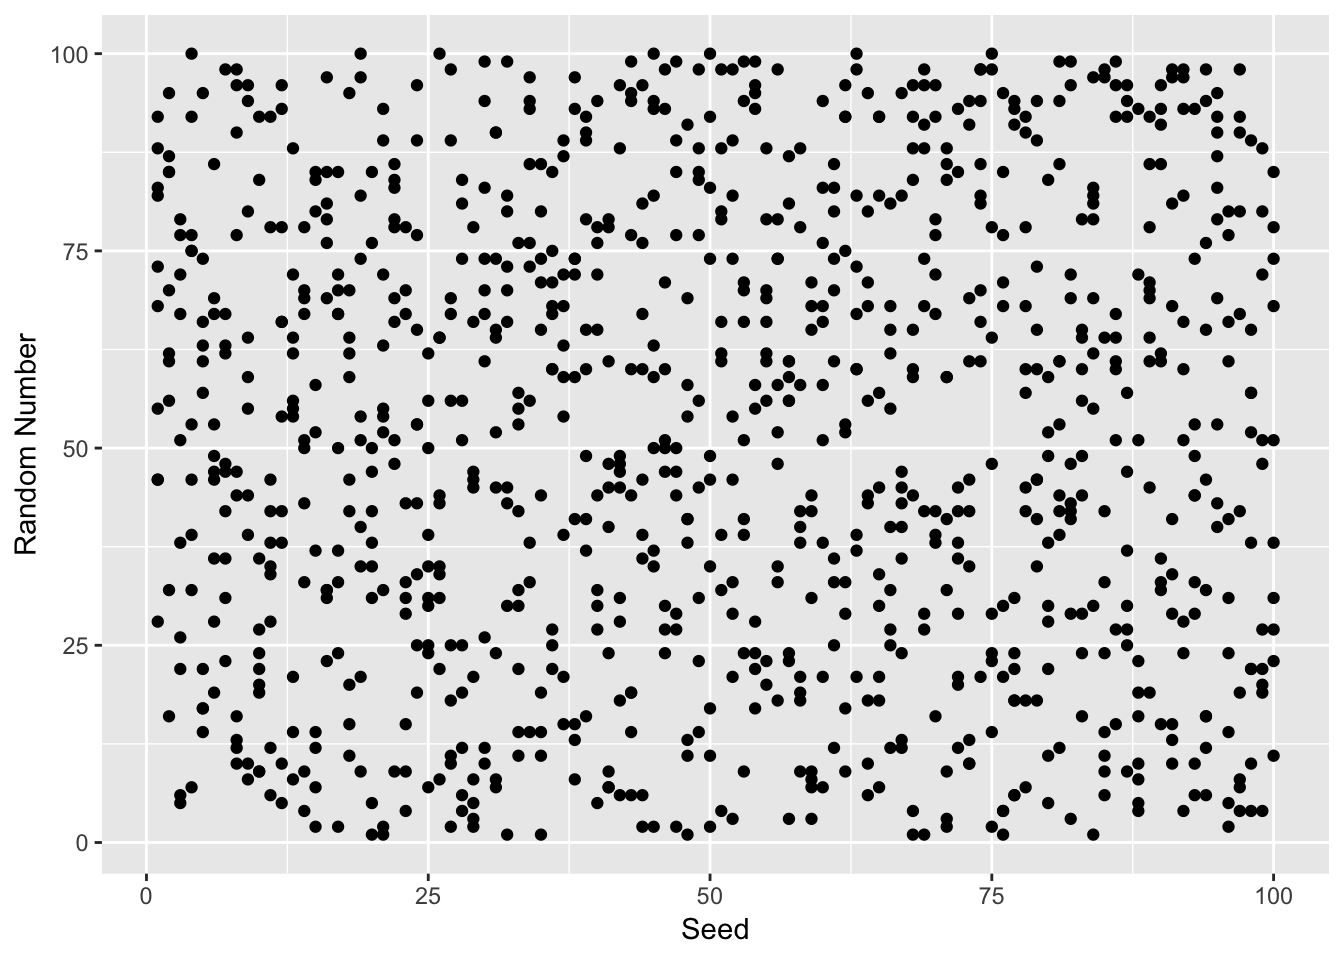
\includegraphics{Homework1_Group3_files/figure-latex/unnamed-chunk-4-1.pdf}

\hypertarget{boxplots}{%
\subsubsection{Boxplots}\label{boxplots}}

In addition to creating histogram distributions, we also elected to use
box-plots to get an idea of the spread of each variable.

\includegraphics{Homework1_Group3_files/figure-latex/unnamed-chunk-5-1.pdf}

The box-plots reveal significant outliers and uniform (zero-only) values
for many of our predictor variables. Outliers will need to imputed if
necessary, and sparse data-sets might need to be dropped.

\hypertarget{variable-plots}{%
\subsubsection{Variable Plots}\label{variable-plots}}

Finally, we wanted to plot scatter plots of each variable versus the
target variable, TARGET\_WINS, to get an idea of the relationship
between them.

\includegraphics{Homework1_Group3_files/figure-latex/unnamed-chunk-6-1.pdf}

The plots indicate some clear relationships, such as hitting more
doubles or more home runs clearly improves the number of wins.

Overall, although our plots indicate some interesting relationships
between our variables, they also reveal some significant issues with the
data.

For instance, most of the predictor variables are skewed or non-normally
distributed, and will need to be transformed. Additionally, there are
many data points that contain missing data that will need to be either
imputed or discarded. It also appears we have some missing data encoded
as 0 and some nonsensical outliers.

There is a team with 0 wins in the dataset. This seems unlikely. Many of
the hitting categories include teams at 0; it is unlikely that a team
hit 0 home runs over the course of a season.

The pitching variables also include many 0's, for instance there are
multiple teams with 0 strikeouts by their pitchers over the season which
is extremely unlikely. The pitching data also includes strange outliers
such as a team logging 20,000 strikeouts, that would be an average of
160 strikeouts per game which is impossible. Also team pitching walks
and team pitching hits have strange outliers.

Lastly, the error variable makes little sense. From our experience
watching baseball, teams usually score 2 or less errors per game, which
would lead to an overall team error of approximately 320 over the course
of a season, which does not match the scale of the error variable. It is
possible that errors have become much less frequent over time which
would account for the high error data.

\hypertarget{missing-data}{%
\subsubsection{Missing Data}\label{missing-data}}

When we initially viewed the first few rows of the raw data, we already
noticed missing data. Let's assess which fields have missing data.

\begin{verbatim}
##    values         ind
## 1   91.61 BATTING_HBP
## 2   33.92  BASERUN_CS
## 3   12.57 FIELDING_DP
## 4    5.76  BASERUN_SB
## 5    4.48  BATTING_SO
## 6    4.48 PITCHING_SO
## 7    0.00 TARGET_WINS
## 8    0.00   BATTING_H
## 9    0.00  BATTING_2B
## 10   0.00  BATTING_3B
## 11   0.00  BATTING_HR
## 12   0.00  BATTING_BB
## 13   0.00  PITCHING_H
## 14   0.00 PITCHING_HR
## 15   0.00 PITCHING_BB
## 16   0.00  FIELDING_E
\end{verbatim}

Notice that \textasciitilde91.6\% of the rows are missing from the
BATTING\_HBP field - we will just drop this column from consideration.
The columns BASERUN\_CS (base run caught stealing) and BASERUN\_SB
(stolen bases) both have missing values. According to baseball history,
stolen bases weren't tracked officially until 1887, so some of the
missing data could be from 1871-1886. We will impute those values. There
are a high percentage of missing BATTING\_SO (batter strike outs) and
PITCHING\_SO (pitching strike outs) which seem highly unlikely - we will
also impute those missing values. We have chosen to impute missing
values with the median value of the feature.

\hypertarget{feature-target-correlations}{%
\subsubsection{Feature-Target
Correlations}\label{feature-target-correlations}}

With our missing data imputed correctly, we can now build off the
scatter plots from above to quantify the correlations between our target
variable and predictor variable. We will want to choose those with
stronger positive or negative correlations. Features with correlations
closer to zero will probably not provide any meaningful information on
explaining wins by a team.

\begin{verbatim}
##          values         ind
## 1   0.383313355   BATTING_H
## 2   0.285964582  BATTING_2B
## 3   0.225471523  BATTING_BB
## 4   0.186326615 PITCHING_HR
## 5   0.173551988  BATTING_HR
## 6   0.164738136 PITCHING_BB
## 7   0.139073830  BATTING_3B
## 8   0.121110012  BASERUN_SB
## 9   0.105034615  PITCHING_H
## 10  0.009835166  BASERUN_CS
## 11 -0.030050754 FIELDING_DP
## 12 -0.037712096  BATTING_SO
## 13 -0.083637577  FIELDING_E
## 14 -0.089519609 PITCHING_SO
\end{verbatim}

BATTING\_H and BATTING\_2B have the highest correlation (positive) with
TOTAL\_WINs; this makes sense given that more hits means more
points/runs, and thus likelihood to win the game. The other variables
have weak or slightly negative correlation, which can imply they might
have little predictive power.

\hypertarget{multicolinearity}{%
\subsubsection{Multicolinearity}\label{multicolinearity}}

One problem that can occur with multi-variable regression is correlation
between variables, or multicolinearity. A quick check is to run
correlations between variables.

\includegraphics{Homework1_Group3_files/figure-latex/unnamed-chunk-10-1.pdf}

We can see that some variables are highly correlated with one another,
such as PITCHING\_BB and BATTING\_BB. When we start considering features
for our models, we'll need to account for the correlations between
features and avoid including pairs with strong correlations.

As a note, this dataset is challenging as many of the predictive
features go hand-in-hand with other feature and multicolinearity will be
a problem. Better teams will see all positive features go up and
negative features go down and vice versa. Many features are also
inherently associated, for example, as batter strike outs increase, we
would expect a decrease in hit metrics. As Base Hits increase, we would
expect to see increases in the 2B, 3B and 4B columns, etc.

\hypertarget{data-preparation}{%
\subsection{2. Data Preparation}\label{data-preparation}}

To summarize our data preparation and exploration, we can distinguish
our findings into a few categories below:

\hypertarget{removed-fields}{%
\subsubsection{Removed Fields}\label{removed-fields}}

We removed the BATTING\_HBP field as it was missing \textgreater90\% of
the data and the INDEX field as it offers no information for a model.

\hypertarget{missing-values}{%
\subsubsection{Missing Values}\label{missing-values}}

There were missing values found in BASERUN\_CS (Caught Stolen Bases),
FIELDING\_DP (Double plays), BASERUN\_SB (Stolen Bases), BATTING\_SO
(Batter Strike outs), PITCHING\_SO (Pitcher Strike outs) so we decided
to replace these missing values with their corresponding median values.
It is highly unlikely that teams had none of these during an entire
season.

\hypertarget{outliers}{%
\subsubsection{Outliers}\label{outliers}}

There are unreasonable outliers found in PITCHING\_SO (pitching
strikeouts), PITCHING\_H (allowed hits per game), PITCHING\_BB (walks),
and FIELDING\_E (fielding errors) that exceed what is reasonable or
possible given standard game length. While specific games might have
outliers (e.g.~in a game with extra innings), we wouldn't expect the
totals per season to allow for outliers in every game. Given this, we
will replace any outliers with the median for the data set. Limits we
set included: \textgreater{} 4000 PITCHING\_SO (25 strikeouts per game),
\textgreater{} 5000 PITCHING\_H (30 hits allowed per game),
\textgreater{} 2000 PITCHING\_BB (13 walks per game) and \textgreater{}
480 FIELDING\_E (3 errors per game).

\hypertarget{transform-non-normal-variables}{%
\subsubsection{Transform non-normal
variables}\label{transform-non-normal-variables}}

Finally, as mentioned earlier in our data exploration, and our findings
from our histogram plots, we can see that some of our variables are
highly skewed. To address this, we decided to perform some
transformations to make them more normally distributed. Here are some
plots to demonstrate the changes in distributions before and after the
transformations:

\includegraphics{Homework1_Group3_files/figure-latex/unnamed-chunk-11-1.pdf}

\hypertarget{finalizing-the-dataset-for-model-building}{%
\subsubsection{Finalizing the dataset for model
building}\label{finalizing-the-dataset-for-model-building}}

With our transformations complete, we can now add these into our
\texttt{clean\_df} dataframe and continue on to build our models.

\hypertarget{build-models}{%
\subsection{3. Build Models}\label{build-models}}

\emph{Using the training data set, build at least three different
multiple linear regression models, using different variables (or the
same variables with different transformations). Since we have not yet
covered automated variable selection methods, you should select the
variables manually (unless you previously learned Forward or Stepwise
selection, etc.). Since you manually selected a variable for inclusion
into the model or exclusion into the model, indicate why this was done.}
\emph{Discuss the coefficients in the models, do they make sense? For
example, if a team hits a lot of Home Runs, it would be reasonably
expected that such a team would win more games. However, if the
coefficient is negative (suggesting that the team would lose more
games), then that needs to be discussed. Are you keeping the model even
though it is counter intuitive? Why? The boss needs to know.}

\hypertarget{model-building-methodology}{%
\subsubsection{Model-building
methodology}\label{model-building-methodology}}

With a solid understanding of our dataset at this point, and with our
data cleaned, we can now start to build out some of our multiple linear
regression models.

First, we decided to split our cleaned dataset into a training and
testing set (80\% training, 20\% testing). Then, using our training
dataset, we decided to run a multiple linear regression model (Model
\#1) that included all non-transformed features that we hadn't removed
following our data cleaning process mentioned above. Next, in Model \#2,
to help us select the optimal set of features, we ran the
\texttt{stepAIC} function in R to perform stepwise selection on our
initial model to help reduce the number of features and address some of
our multicollinearity issues from Model \#1 (explained more below).
Finally, our last model (Model \#3) included all data from our cleaned
dataset, but also contained some of our transformed features in
replacement of their non-transformed counterparts. Additionally, we ran
this model through stepwise selection as well to determine the optimal
set of features and to reduce multicollinearity as much as possible.

\hypertarget{examining-our-model-coefficients}{%
\subsubsection{Examining our model
coefficients}\label{examining-our-model-coefficients}}

Throughout our model-building process, we noticed that many of our model
outputs yielded a few coefficient values that seemed to contradict our
initial estimates. For instance, in Model \#1:

\textbf{Negative values for coefficients that we'd expect to be
positive}

\begin{itemize}
\tightlist
\item
  BATTING\_2B - logically more doubles hit by batters would increase the
  likelihood of winning more games\\
\item
  BATTING\_HR - logically more homeruns hit by batters would increase
  the likelihood of winning more games\\
\item
  PITCHING\_SO - logically more strikeouts thrown by pitchers would
  increase the likelihood of winning more games\\
\item
  FIELDING\_DP - logically more double plays turned by a team would
  increase the likelihood of winning more games
\end{itemize}

\textbf{Positive values for coefficients that we'd expect to be
negative}

\begin{itemize}
\tightlist
\item
  BATTING\_SO - logically more strikeouts by batters would lead to less
  of a likelihood of winning more games\\
\item
  PITCHING\_H - logically more hits given up by pitchers would lead to
  less of a likelihood of winning more games\\
\item
  PITCHING\_HR - logically more homeruns given up by pitchers would lead
  to less of a likelihood of winning more games
\end{itemize}

This is a trend we saw throughout the three models that we built,
although Model \#3 was able to adjust for this better than our first two
models -- we can likely attribute this phenomenon to multicollinearity.
Since we noticed in our initial data exploration that many variables in
the dataset were highly correlated with one another (i.e.~BATTING\_2B
and BATTING\_HR), this phenomenon likely is increasing the variance of
the coefficient estimates, making them difficult to interpret (and in
some cases such as the features listed above, they are switching the
signs). This was also supported by our Variance Inflation Factor (VIF)
tests, which showed high values for features such as BATTING\_HR,
BATTING\_SO, PITCHING\_HR, and PITCHING\_SO. In our final model (Model
\#3), we made sure to keep this in mind in order to get a better handle
on our coefficients and reduce multicollinearity -- mainly, we removed
certain variables that had high VIF scores through our stepwise
selection process. Later in our discussion, we'll discuss whether or not
we'd keep our final model based on this issue.

\hypertarget{model-1}{%
\subsubsection{Model 1}\label{model-1}}

Below is our initial multiple linear regression model that includes all
features from our cleaned dataset.

\begin{verbatim}
## 
## Call:
## lm(formula = TARGET_WINS ~ BATTING_H + BATTING_2B + BATTING_3B + 
##     BATTING_HR + BATTING_BB + BATTING_SO + BASERUN_SB + BASERUN_CS + 
##     PITCHING_H + PITCHING_HR + PITCHING_BB + PITCHING_SO + FIELDING_E + 
##     FIELDING_DP, data = df_train)
## 
## Residuals:
##     Min      1Q  Median      3Q     Max 
## -61.219  -8.227  -0.078   8.275  64.097 
## 
## Coefficients:
##              Estimate Std. Error t value Pr(>|t|)    
## (Intercept) 19.159307   6.307639   3.037 0.002420 ** 
## BATTING_H    0.045729   0.004176  10.950  < 2e-16 ***
## BATTING_2B  -0.020206   0.010083  -2.004 0.045228 *  
## BATTING_3B   0.098643   0.018671   5.283 1.42e-07 ***
## BATTING_HR  -0.064392   0.033802  -1.905 0.056944 .  
## BATTING_BB   0.062187   0.005419  11.476  < 2e-16 ***
## BATTING_SO   0.006454   0.004455   1.449 0.147609    
## BASERUN_SB   0.016532   0.004656   3.550 0.000394 ***
## BASERUN_CS  -0.008546   0.017416  -0.491 0.623716    
## PITCHING_H   0.002280   0.001022   2.231 0.025803 *  
## PITCHING_HR  0.098044   0.029903   3.279 0.001063 ** 
## PITCHING_BB -0.031403   0.004585  -6.848 1.02e-11 ***
## PITCHING_SO -0.006677   0.003202  -2.085 0.037196 *  
## FIELDING_E  -0.046709   0.005781  -8.080 1.17e-15 ***
## FIELDING_DP -0.141952   0.014887  -9.535  < 2e-16 ***
## ---
## Signif. codes:  0 '***' 0.001 '**' 0.01 '*' 0.05 '.' 0.1 ' ' 1
## 
## Residual standard error: 12.99 on 1806 degrees of freedom
## Multiple R-squared:  0.3143, Adjusted R-squared:  0.309 
## F-statistic: 59.14 on 14 and 1806 DF,  p-value: < 2.2e-16
\end{verbatim}

\begin{verbatim}
##                     2.5 %        97.5 %
## (Intercept)  6.7882721761 31.5303425736
## BATTING_H    0.0375385910  0.0539198420
## BATTING_2B  -0.0399821239 -0.0004299296
## BATTING_3B   0.0620239169  0.1352624539
## BATTING_HR  -0.1306881198  0.0019035737
## BATTING_BB   0.0515586246  0.0728152929
## BATTING_SO  -0.0022838297  0.0151917050
## BASERUN_SB   0.0073994809  0.0256640050
## BASERUN_CS  -0.0427037715  0.0256123654
## PITCHING_H   0.0002756037  0.0042835297
## PITCHING_HR  0.0393959474  0.1566927835
## PITCHING_BB -0.0403967131 -0.0224100318
## PITCHING_SO -0.0129569170 -0.0003966439
## FIELDING_E  -0.0580462638 -0.0353716216
## FIELDING_DP -0.1711508024 -0.1127541087
\end{verbatim}

\includegraphics{Homework1_Group3_files/figure-latex/unnamed-chunk-13-1.pdf}

We can explicitly call out our variable importances using the Caret
package which will determine our feature importance for each of the
multiple linear regression models individually.

We also examine the VIF of our variables to check for multicolinearity
in the model.

\includegraphics{Homework1_Group3_files/figure-latex/unnamed-chunk-14-1.pdf}

\begin{verbatim}
## [1] "VIF scores of predictors"
\end{verbatim}

\begin{verbatim}
##   BATTING_H  BATTING_2B  BATTING_3B  BATTING_HR  BATTING_BB  BATTING_SO 
##    3.982149    2.392001    2.908248   44.695422    4.722647   12.426490 
##  BASERUN_SB  BASERUN_CS  PITCHING_H PITCHING_HR PITCHING_BB PITCHING_SO 
##    1.700422    1.122540    2.059995   35.894247    3.740457    7.148733 
##  FIELDING_E FIELDING_DP 
##    1.993090    1.438791
\end{verbatim}

\hypertarget{model-2}{%
\subsubsection{Model 2}\label{model-2}}

In our second model, below, we decided to use stepwise selection in
order to help us determine the optimal set of features from our
original, cleaned dataset.

\begin{verbatim}
## 
## Call:
## lm(formula = TARGET_WINS ~ BATTING_H + BATTING_2B + BATTING_3B + 
##     BATTING_HR + BATTING_BB + BATTING_SO + BASERUN_SB + PITCHING_H + 
##     PITCHING_HR + PITCHING_BB + PITCHING_SO + FIELDING_E + FIELDING_DP, 
##     data = df_train)
## 
## Residuals:
##     Min      1Q  Median      3Q     Max 
## -61.233  -8.200  -0.015   8.302  64.234 
## 
## Coefficients:
##              Estimate Std. Error t value Pr(>|t|)    
## (Intercept) 18.720588   6.242634   2.999 0.002747 ** 
## BATTING_H    0.045677   0.004174  10.943  < 2e-16 ***
## BATTING_2B  -0.020475   0.010066  -2.034 0.042098 *  
## BATTING_3B   0.099109   0.018643   5.316 1.19e-07 ***
## BATTING_HR  -0.062516   0.033578  -1.862 0.062794 .  
## BATTING_BB   0.062017   0.005407  11.470  < 2e-16 ***
## BATTING_SO   0.006336   0.004448   1.425 0.154462    
## BASERUN_SB   0.016165   0.004595   3.518 0.000446 ***
## PITCHING_H   0.002305   0.001020   2.260 0.023947 *  
## PITCHING_HR  0.097186   0.029846   3.256 0.001150 ** 
## PITCHING_BB -0.031213   0.004568  -6.833 1.13e-11 ***
## PITCHING_SO -0.006602   0.003198  -2.064 0.039115 *  
## FIELDING_E  -0.046569   0.005772  -8.068 1.29e-15 ***
## FIELDING_DP -0.141912   0.014884  -9.534  < 2e-16 ***
## ---
## Signif. codes:  0 '***' 0.001 '**' 0.01 '*' 0.05 '.' 0.1 ' ' 1
## 
## Residual standard error: 12.99 on 1807 degrees of freedom
## Multiple R-squared:  0.3143, Adjusted R-squared:  0.3093 
## F-statistic:  63.7 on 13 and 1807 DF,  p-value: < 2.2e-16
\end{verbatim}

\includegraphics{Homework1_Group3_files/figure-latex/unnamed-chunk-15-1.pdf}

\includegraphics{Homework1_Group3_files/figure-latex/unnamed-chunk-16-1.pdf}

\begin{verbatim}
## [1] "VIF scores of predictors"
\end{verbatim}

\begin{verbatim}
##   BATTING_H  BATTING_2B  BATTING_3B  BATTING_HR  BATTING_BB  BATTING_SO 
##    3.979587    2.384946    2.900725   44.123572    4.703397   12.390288 
##  BASERUN_SB  PITCHING_H PITCHING_HR PITCHING_BB PITCHING_SO  FIELDING_E 
##    1.656576    2.054487   35.771529    3.713621    7.132372    1.988251 
## FIELDING_DP 
##    1.438747
\end{verbatim}

\hypertarget{model-3}{%
\subsubsection{Model 3}\label{model-3}}

In our third model, we decided to utilize some of our transformed
variables to compare against our initial model. Additionally, similar to
model 2, we used stepwise selection to determine feature importance and
select the simplest model possible.

\begin{verbatim}
## 
## Call:
## lm(formula = TARGET_WINS ~ BATTING_H + BATTING_2B + BATTING_3B_transform + 
##     BATTING_HR_transform + BATTING_BB + BATTING_SO + BASERUN_SB_transform + 
##     BASERUN_CS + PITCHING_H + PITCHING_HR + PITCHING_BB_transform + 
##     PITCHING_SO_transform + FIELDING_E_transform + FIELDING_DP, 
##     data = df_train)
## 
## Residuals:
##     Min      1Q  Median      3Q     Max 
## -58.076  -8.145   0.051   8.272  61.294 
## 
## Coefficients:
##                         Estimate Std. Error t value Pr(>|t|)    
## (Intercept)            8.476e+00  2.086e+01   0.406  0.68449    
## BATTING_H              4.645e-02  4.162e-03  11.162  < 2e-16 ***
## BATTING_2B            -2.051e-02  1.004e-02  -2.044  0.04113 *  
## BATTING_3B_transform   6.305e+00  1.013e+00   6.226 5.92e-10 ***
## BATTING_HR_transform  -5.733e-02  3.423e-01  -0.168  0.86699    
## BATTING_BB             6.444e-02  6.292e-03  10.241  < 2e-16 ***
## BATTING_SO            -3.839e-03  4.378e-03  -0.877  0.38064    
## BASERUN_SB_transform   2.106e+00  6.474e-01   3.252  0.00117 ** 
## BASERUN_CS            -7.216e-03  1.811e-02  -0.398  0.69038    
## PITCHING_H             1.226e-04  1.077e-03   0.114  0.90934    
## PITCHING_HR            4.067e-02  2.032e-02   2.002  0.04547 *  
## PITCHING_BB_transform -1.649e+01  2.685e+00  -6.140 1.01e-09 ***
## PITCHING_SO_transform  1.557e+00  2.857e+00   0.545  0.58575    
## FIELDING_E_transform   2.789e+02  3.613e+01   7.720 1.92e-14 ***
## FIELDING_DP           -1.384e-01  1.530e-02  -9.049  < 2e-16 ***
## ---
## Signif. codes:  0 '***' 0.001 '**' 0.01 '*' 0.05 '.' 0.1 ' ' 1
## 
## Residual standard error: 13.04 on 1806 degrees of freedom
## Multiple R-squared:  0.309,  Adjusted R-squared:  0.3037 
## F-statistic: 57.69 on 14 and 1806 DF,  p-value: < 2.2e-16
\end{verbatim}

\begin{verbatim}
##                               2.5 %        97.5 %
## (Intercept)           -32.428934106  4.938152e+01
## BATTING_H               0.038288318  5.461267e-02
## BATTING_2B             -0.040197396 -8.267731e-04
## BATTING_3B_transform    4.319302256  8.291619e+00
## BATTING_HR_transform   -0.728612807  6.139452e-01
## BATTING_BB              0.052098342  7.678028e-02
## BATTING_SO             -0.012425392  4.747207e-03
## BASERUN_SB_transform    0.835919512  3.375463e+00
## BASERUN_CS             -0.042738724  2.830686e-02
## PITCHING_H             -0.001988975  2.234216e-03
## PITCHING_HR             0.000821262  8.052069e-02
## PITCHING_BB_transform -21.754732546 -1.122123e+01
## PITCHING_SO_transform  -4.045693300  7.160179e+00
## FIELDING_E_transform  208.032462919  3.497396e+02
## FIELDING_DP            -0.168440098 -1.084293e-01
\end{verbatim}

\includegraphics{Homework1_Group3_files/figure-latex/unnamed-chunk-17-1.pdf}

\begin{verbatim}
## 
## Call:
## lm(formula = TARGET_WINS ~ BATTING_H + BATTING_2B + BATTING_3B_transform + 
##     BATTING_BB + BASERUN_SB_transform + PITCHING_HR + PITCHING_BB_transform + 
##     FIELDING_E_transform + FIELDING_DP, data = df_train)
## 
## Residuals:
##     Min      1Q  Median      3Q     Max 
## -57.878  -8.218  -0.006   8.246  60.682 
## 
## Coefficients:
##                         Estimate Std. Error t value Pr(>|t|)    
## (Intercept)             6.879163  13.255656   0.519 0.603852    
## BATTING_H               0.048322   0.003235  14.938  < 2e-16 ***
## BATTING_2B             -0.024057   0.009552  -2.518 0.011871 *  
## BATTING_3B_transform    6.489195   0.995661   6.517 9.24e-11 ***
## BATTING_BB              0.060577   0.004561  13.283  < 2e-16 ***
## BASERUN_SB_transform    1.892989   0.565988   3.345 0.000841 ***
## PITCHING_HR             0.034267   0.008648   3.962 7.71e-05 ***
## PITCHING_BB_transform -15.064064   2.166169  -6.954 4.93e-12 ***
## FIELDING_E_transform  280.475431  34.237604   8.192 4.80e-16 ***
## FIELDING_DP            -0.138331   0.014738  -9.386  < 2e-16 ***
## ---
## Signif. codes:  0 '***' 0.001 '**' 0.01 '*' 0.05 '.' 0.1 ' ' 1
## 
## Residual standard error: 13.03 on 1811 degrees of freedom
## Multiple R-squared:  0.3083, Adjusted R-squared:  0.3049 
## F-statistic:  89.7 on 9 and 1811 DF,  p-value: < 2.2e-16
\end{verbatim}

\includegraphics{Homework1_Group3_files/figure-latex/unnamed-chunk-17-2.pdf}

We can assess variable importance of our model with our original dataset
(model 2) to our transformed dataset (model 3) as shown below. We notice
that ``Batting\_BB'' and ``Batting\_H'' are much closer together in
terms of weight in predicting target\_wins than in model 1
(pre-transformed)

\includegraphics{Homework1_Group3_files/figure-latex/unnamed-chunk-18-1.pdf}

\begin{verbatim}
## [1] "VIF scores of predictors"
\end{verbatim}

\begin{verbatim}
##             BATTING_H            BATTING_2B  BATTING_3B_transform 
##              2.374987              2.133918              2.575616 
##            BATTING_BB  BASERUN_SB_transform           PITCHING_HR 
##              3.324985              1.333406              2.984269 
## PITCHING_BB_transform  FIELDING_E_transform           FIELDING_DP 
##              2.784566              2.238671              1.401629
\end{verbatim}

\hypertarget{model-selection-analysis}{%
\subsection{4. Model Selection \&
Analysis}\label{model-selection-analysis}}

\emph{For the multiple linear regression model, will you use a metric
such as Adjusted R2, RMSE, etc.? Be sure to explain how you can make
inferences from the model, discuss multi-collinearity issues (if any),
and discuss other relevant model output. Using the training data set,
evaluate the multiple linear regression model based on (a) mean squared
error, (b) R2, (c) F-statistic, and (d) residual plots. Make predictions
using the evaluation data set.}

The following table discusses each of the model performance metrics on
the training dataset. These values indicate there is a minor improvement
in model performance after applying transformations and selecting for
significant parameters.

All models achieved a positive adjusted R\^{}2 pointing to a
weakly-positive relationship between the target variable TOTAL\_WINs and
the model predictor variables.

From the previous section and residual diagnostics (both the residual
histogram and QQ plot)--all three models have normally distributed
residuals with mean 0. There appears to be no heteroskedasticity
(non-constant variance) or serial-correlation within the residuals--thus
strictly from a linear regression perspective, none of the assumptions
are violated and thus we can make inferential predictions based on our
model.

Next looking at the F-statistic for all models were large and achieved a
statistically significant p-value than than a default alpha of .05; thus
for all three models the Null hypothesis that is rejected that 0s for
our regression coefficients would fit the data better.

From the exploratory data analysis we saw that many of the predictor
variables were correlated with each other--this makes sense given that
baseball is a team sport, and thus different position scoring/runs helps
contribute to wins. However this could be an issue from a
multicolinearity, that can lead to unstable regression fits. From the
previous section we used VIF (Variable Inflation Factor) to gauge better
models by preferring VIF values less than 5.

\begin{table}[H]
\centering
\begin{tabular}{l|r|r|r}
\hline
  & RSE & Adj.R2 & F.Statistic\\
\hline
Model 1 & 12.99105 & 0.3090296 & 59.14120\\
\hline
Model 2 & 12.98832 & 0.3093199 & 63.69877\\
\hline
Model 3 & 13.02985 & 0.3048964 & 89.70165\\
\hline
\end{tabular}
\end{table}

The following figure represents the performance of 3 of the models on
both the testing and on the training dataset. for this multiple linear
regression problem, the adjusted R2 value was used as the metric for
performance on predicting the target wins.

\includegraphics{Homework1_Group3_files/figure-latex/unnamed-chunk-20-1.pdf}

The analysis shows the following results:

Model 1 - This model is based on the all predictors on an un-transformed
dataset. Results for this model provided an R\^{}2 of about of 0.31 on
the training set and 0.3 on the testing dataset.

Model 2 - This model is based on a subset of significant predictors on
an un-transformed dataset. Results for this model provided an R\^{}2 of
about of 0.31 on the training set and 0.31 on the testing dataset.

Model 3 - This model is based on a subset of significant predictors on
an transformed dataset. Results for this model provided an R\^{}2 of
about of 0.31 on the training set and 0.31 on the testing dataset.

\hypertarget{model-of-choice}{%
\subsubsection{Model of choice}\label{model-of-choice}}

Based on these analyses, Model 2 and Model 3 both performed marginally
better than Model 1 and could be selected as the linear model of choice
when looking at adjusted R2. However, there is greater statistical
significance under the third model relative to the others and uses less
unnecessary variables to compute our prediction without sacrificing much
in terms of adjusted R\^{}2 value. Additionally, Model 3 seems to have
lower VIF scores than Models 1 and 2. Because of these factors, as well
as its better adjustment for multicollinearity (we noticeably saw less
sign-flipping in coefficients), model 3 would be the model of choice.

\hypertarget{references}{%
\subsection{References}\label{references}}

\begin{itemize}
\tightlist
\item
  A Modern Approach to Regression with R: Simon Sheather
\item
  Linear Models with R: Julian Faraway.
\item
  R package vignette,
  \href{https://cran.r-project.org/web/packages/mixtools/vignettes/mixtools.pdf}{mixtools:
  An R Package for Analyzing Finite Mixture Models}
\item
  \href{https://statisticsbyjim.com/regression/ols-linear-regression-assumptions/}{7
  Classic OLS assumptions}
\item
  \href{https://online.stat.psu.edu/stat462/node/180/}{Detecting
  Multicolinearity with VIF}
\end{itemize}

\hypertarget{appendix}{%
\subsection{Appendix}\label{appendix}}

\hypertarget{a.-moneyball-dataset-columns}{%
\subsubsection{A. Moneyball Dataset
Columns}\label{a.-moneyball-dataset-columns}}

\begin{itemize}
\tightlist
\item
  INDEX: Identification Variable(Do not use)
\item
  TARGET\_WINS: Number of wins
\item
  TEAM\_BATTING\_H : Base Hits by batters (1B,2B,3B,HR)
\item
  TEAM\_BATTING\_2B: Doubles by batters (2B)
\item
  TEAM\_BATTING\_3B: Triples by batters (3B)
\item
  TEAM\_BATTING\_HR: Home runs by batters (4B)
\item
  TEAM\_BATTING\_BB: Walks by batters
\item
  TEAM\_BATTING\_HBP: Batters hit by pitch (get a free base)
\item
  TEAM\_BATTING\_SO: Strikeouts by batters
\item
  TEAM\_BASERUN\_SB: Stolen bases
\item
  TEAM\_BASERUN\_CS: Caught stealing
\item
  TEAM\_FIELDING\_E: Errors
\item
  TEAM\_FIELDING\_DP: Double Plays
\item
  TEAM\_PITCHING\_BB: Walks allowed
\item
  TEAM\_PITCHING\_H: Hits allowed
\item
  TEAM\_PITCHING\_HR: Homeruns allowed
\item
  TEAM\_PITCHING\_SO: Strikeouts by pitchers
\end{itemize}

\hypertarget{r-code}{%
\subsubsection{R Code}\label{r-code}}

\begin{verbatim}
# =====================================================================================
# Load Libraries and Define Helper functions 
# =====================================================================================

library(MASS)
library(rpart.plot)
library(ggplot2)
library(ggfortify)
library(gridExtra)
library(forecast)
library(fpp2)
library(fma)
library(kableExtra)
library(e1071)
library(mlbench)
library(ggcorrplot)
library(DataExplorer)
library(timeDate)
library(caret)
library(GGally)
library(corrplot)
library(RColorBrewer)
library(tibble)
library(tidyr)
library(tidyverse)
library(dplyr)
library(reshape2)
library(mixtools)
library(tidymodels)
library(ggpmisc)
library(regclass)

#' Print a side-by-side Histogram and QQPlot of Residuals
#'
#' @param model A model
#' @examples
#' residPlot(myModel)
#' @return null
#' @export
residPlot <- function(model) {
  # Make sure a model was passed
  if (is.null(model)) {
    return
  }
  
  layout(matrix(c(1,1,2,3), 2, 2, byrow = TRUE))
  plot(residuals(model))
  hist(model[["residuals"]], freq = FALSE, breaks = "fd", main = "Residual Histogram",
       xlab = "Residuals",col="lightgreen")
  lines(density(model[["residuals"]], kernel = "ep"),col="blue", lwd=3)
  curve(dnorm(x,mean=mean(model[["residuals"]]), sd=sd(model[["residuals"]])), col="red", lwd=3, lty="dotted", add=T)
  qqnorm(model[["residuals"]], main = "Residual Q-Q plot")
  qqline(model[["residuals"]],col="red", lwd=3, lty="dotted")
  par(mfrow = c(1, 1))
}

#' Print a Variable Importance Plot for the provided model
#'
#' @param model The model
#' @param chart_title The Title to show on the plot
#' @examples
#' variableImportancePlot(myLinearModel, 'My Title)
#' @return null
#' @export
variableImportancePlot <- function(model=NULL, chart_title='Variable Importance Plot') {
  # Make sure a model was passed
  if (is.null(model)) {
    return
  }
  
  # use caret and gglot to print a variable importance plot
  varImp(model) %>% as.data.frame() %>% 
    ggplot(aes(x = reorder(rownames(.), desc(Overall)), y = Overall)) +
    geom_col(aes(fill = Overall)) +
    theme(panel.background = element_blank(),
          panel.grid = element_blank(),
          axis.text.x = element_text(angle = 90)) +
    scale_fill_gradient() +
    labs(title = chart_title,
         x = "Parameter",
         y = "Relative Importance")
}


#' Print a Facet Chart of histograms
#'
#' @param df Dataset
#' @param box Facet size (rows)
#' @examples
#' histbox(my_df, 3)
#' @return null
#' @export
histbox <- function(df, box) {
    par(mfrow = box)
    ndf <- dimnames(df)[[2]]
    
    for (i in seq_along(ndf)) {
            data <- na.omit(unlist(df[, i]))
            hist(data, breaks = "fd", main = paste("Histogram of", ndf[i]),
                 xlab = ndf[i], freq = FALSE)
            lines(density(data, kernel = "ep"), col = 'red')
    }
    
    par(mfrow = c(1, 1))
}

#' Extract key performance results from a model
#'
#' @param model A linear model of interest
#' @examples
#' model_performance_extraction(my_model)
#' @return data.frame
#' @export
model_performance_extraction <- function(model=NULL) {
  # Make sure a model was passed
  if (is.null(model)) {
    return
  }
  
  data.frame("RSE" = model$sigma,
             "Adj R2" = model$adj.r.squared,
             "F-Statistic" = model$fstatistic[1])
}

# =====================================================================================
# Load Data set
# =====================================================================================

# Load Moneyball baseball dataset
df <- read.csv('datasets/moneyball-training-data.csv')
df_eval <- read.csv('datasets/moneyball-evaluation-data.csv')

# Remove superfluous TEAM_ from column names
names(df) <- names(df) %>% 
  str_replace_all('TEAM_', '')
  
# Drop the INDEX column - this won't be useful
df <- df %>% 
  dplyr::select(-INDEX)

# =====================================================================================
# Summary Stats 
# =====================================================================================

# Display summary statistics
summary(df)

# =====================================================================================
# Distributions 
# =====================================================================================

# Prepare data for ggplot
gather_df <- df %>% 
  gather(key = 'variable', value = 'value')

# Histogram plots of each variable
ggplot(gather_df) + 
  geom_histogram(aes(x=value, y = ..density..), bins=30) + 
  geom_density(aes(x=value), color='blue') +
  facet_wrap(. ~variable, scales='free', ncol=4)

# Select BATTING_SO column and remove any missing data
df_mix <- df %>% 
  dplyr::select(BATTING_SO) %>%
  drop_na()

# Calculate mixed distributions for BATTING_SO
batting_so_mix <- normalmixEM(df_mix$BATTING_SO, 
                              lambda = .5, 
                              mu = c(400, 1200), 
                              sigma = 5, 
                              maxit=60)

# Simple plot to illustrate possible bimodal mix of groups
plot(batting_so_mix, 
     whichplots = 2,
     density = TRUE, 
     main2 = "BATTING_SO Possible Distributions", 
     xlab2 = "BATTING_SO")
     
# =====================================================================================
# Boxplots 
# =====================================================================================

# Prepare data for ggplot
gather_df <- df %>% 
  gather(key = 'variable', value = 'value')

# Boxplots for each variable
ggplot(gather_df, aes(variable, value)) + 
  geom_boxplot() + 
  facet_wrap(. ~variable, scales='free', ncol=6)

# =====================================================================================
# Variable Plots
# =====================================================================================
  
# Plot scatter plots of each variable versus the target variable
featurePlot(df[,2:ncol(df)], df[,1], pch = 20)

# =====================================================================================
# Missing Data 
# =====================================================================================

# Identify missing data by Feature and display percent breakout
missing <- colSums(df %>% sapply(is.na))
missing_pct <- round(missing / nrow(df) * 100, 2)
stack(sort(missing_pct, decreasing = TRUE))

# Drop the BATTING_HBP field
df <- df %>% 
  select(-BATTING_HBP)

# We have chosen to impute the median as there are strong outliers that may skew the mean. Could revisit for advanced imputation via prediction later.
no_outlier_df <- df

# 4000 strikeouts is an average of 25 strikeouts per game, which is ridiculous.
no_outlier_df$PITCHING_SO <- ifelse(no_outlier_df$PITCHING_SO > 4000, NA, no_outlier_df$PITCHING_SO)

# 5000 hits is an average of 30 hits allowed per game, which is also ridiculous.
no_outlier_df$PITCHING_H <- ifelse(no_outlier_df$PITCHING_H > 5000, NA, no_outlier_df$PITCHING_H)

# 2000 walks is an average of 13 walks per game which is unlikely.
no_outlier_df$PITCHING_BB <- ifelse(no_outlier_df$PITCHING_BB > 2000, NA, no_outlier_df$PITCHING_BB)

# more than 480 errors is an average of 3 per game which is unlikely.
no_outlier_df$FIELDING_E <- ifelse(no_outlier_df$FIELDING_E > 480, NA, no_outlier_df$FIELDING_E)

clean_df <- no_outlier_df %>% 
  impute(what = 'median') %>% as.data.frame()

# From the plots, the team with 0 wins has 0 in multiple other categories. I believe this is missing data, not valid data.
clean_df <- clean_df %>% 
  filter(TARGET_WINS != 0)

gather_clean_df <- clean_df %>% 
  gather(key = 'variable', value = 'value', -TARGET_WINS)

# =====================================================================================
# Feature-Target Correlations 
# =====================================================================================

# Show feature correlations/target by decreasing correlation
stack(sort(cor(clean_df[,1], clean_df[,2:ncol(clean_df)])[,], decreasing=TRUE))

# =====================================================================================
# Multicolinearity 
# =====================================================================================

correlation = cor(clean_df, use = 'pairwise.complete.obs')

corrplot(correlation, 'ellipse', type = 'lower', order = 'hclust',
         col=brewer.pal(n=8, name="RdYlBu"))

# =====================================================================================
# Transform non-normal variables 
# =====================================================================================
         

# created empty data frame to store transformed variables
df_temp <- data.frame(matrix(ncol = 1, nrow = length(clean_df$TARGET_WINS)))

# performed boxcox transformation after identifying proper lambda
df_temp$BATTING_3B <- clean_df$BATTING_3B
batting3b_lambda <- BoxCox.lambda(clean_df$BATTING_3B)
df_temp$BATTING_3B_transform <- log(clean_df$BATTING_3B)

# performed boxcox transformation after identifying proper lambda
df_temp$BATTING_HR <- clean_df$BATTING_HR
battingHR_lambda <- BoxCox.lambda(clean_df$BATTING_HR)
df_temp$BATTING_HR_transform <- BoxCox(clean_df$BATTING_HR, battingHR_lambda)

# performed a log transformation
df_temp$PITCHING_BB <- clean_df$PITCHING_BB
df_temp$PITCHING_BB_transform <- log(clean_df$PITCHING_BB)

# performed a log transformation
df_temp$PITCHING_SO <- clean_df$PITCHING_SO
df_temp$PITCHING_SO_transform <- log(clean_df$PITCHING_SO)

# performed an inverse log transformation
df_temp$FIELDING_E <- clean_df$FIELDING_E
df_temp$FIELDING_E_transform <- 1/log(clean_df$FIELDING_E)

# performed a log transformation
df_temp$BASERUN_SB <- clean_df$BASERUN_SB
df_temp$BASERUN_SB_transform <- log(clean_df$BASERUN_SB)

df_temp <- df_temp[, 2:13]

histbox(df_temp, c(6, 2))

# =====================================================================================
# Final Cleaned Dataframe with transformations
# =====================================================================================

# Build clean dataframe with transformation
clean_df <- data.frame(cbind(clean_df, 
                        BATTING_3B_transform = df_temp$BATTING_3B_transform,
                        BATTING_HR_transform = df_temp$BATTING_HR_transform,
                        BASERUN_SB_transform = df_temp$BASERUN_SB_transform,
                        PITCHING_BB_transform = df_temp$PITCHING_BB_transform,
                        PITCHING_SO_transform = df_temp$PITCHING_SO_transform,
                        FIELDING_E_transform = df_temp$FIELDING_E_transform))

is.na(clean_df) <- sapply(clean_df, is.infinite)

# Impute missing value with the mean
mean = mean(clean_df$BATTING_3B_transform, na.rm = TRUE)
mean2 = mean(clean_df$BASERUN_SB_transform, na.rm = TRUE)
mean3 = mean(clean_df$PITCHING_SO_transform, na.rm = TRUE)

clean_df$BATTING_3B_transform[is.na(clean_df$BATTING_3B_transform)] <- mean
clean_df$BASERUN_SB_transform[is.na(clean_df$BASERUN_SB_transform)] <- mean2
clean_df$PITCHING_SO_transform[is.na(clean_df$PITCHING_SO_transform)] <- mean3

# =====================================================================================
# Model 1 (without stepAIC)
# =====================================================================================

# Splitting the dataset into train/testing set with 80/20 split
set.seed(3)
df_split <- initial_split(clean_df, prop = 0.8)
df_train <- training(df_split)
df_test <- testing(df_split)

# Model 1 - Include all features and leverage stepAIC to help identify ideal features

multi_lm <- lm(TARGET_WINS ~ BATTING_H + BATTING_2B + BATTING_3B + BATTING_HR + BATTING_BB + BATTING_SO + BASERUN_SB + BASERUN_CS + PITCHING_H + PITCHING_HR + PITCHING_BB + PITCHING_SO + FIELDING_E + FIELDING_DP, df_train)
(lm_s <- summary(multi_lm))
confint(multi_lm)
residPlot(lm_s)

# Model 1 - Display Variable feature importance plot
variableImportancePlot(multi_lm, "Model 1 LM Variable Importance")

# model 1 - print variable inflation factor score
print('VIF scores of predictors')

VIF(multi_lm)

# =====================================================================================
# Model 2 (with stepAIC)
# =====================================================================================

# Build model 2 - this is Model 1 with only significant features (using stepAIC)
mult_lm_final <- stepAIC(multi_lm, direction = "both",
                         scope = list(upper = multi_lm, lower = ~ 1),
                         scale = 0, trace = FALSE)
# Display Model 2 Summary
(lmf_s <- summary(mult_lm_final))

# Display Model 2 REsidual plots
residPlot(lmf_s)

# model 2 - Display Variable feature importance plot
variableImportancePlot(mult_lm_final, "Model 2 LM Variable Importance")

# model 2 - print variable inflation factor score
print('VIF scores of predictors')

VIF(mult_lm_final)

# =====================================================================================
# Model 3 (with stepAIC and transformed features)
# =====================================================================================

# Model 3 - Build linear model
multi_lm_2 <- lm(TARGET_WINS ~ BATTING_H + BATTING_2B + BATTING_3B_transform + BATTING_HR_transform + BATTING_BB + BATTING_SO + BASERUN_SB_transform + BASERUN_CS + PITCHING_H + PITCHING_HR + PITCHING_BB_transform + PITCHING_SO_transform + FIELDING_E_transform + FIELDING_DP, df_train)

# Model 3 - Show model summary info
(lm_s_2 <- summary(multi_lm_2))

# Model 3 - Show Confidence and Residual Plots
confint(multi_lm_2)
residPlot(lm_s_2)

# Model 3 - use stepAIC to select significant features
mult_lm_final_2 <- stepAIC(multi_lm_2, direction = "both",
                         scope = list(upper = multi_lm_2, lower = ~ 1),
                         scale = 0, trace = FALSE)

# Model 3 - Show feature importance in final model after stepAIC
variableImportancePlot(mult_lm_final_2, "Model 3 LM Variable Importance")

# Model 3 - show Variance Inflation Factor score
print('VIF scores of predictors')

VIF(mult_lm_final_2)

# =====================================================================================
# Select Models
# =====================================================================================

# Build summary table with each model performance metrics
SummaryTable <- bind_rows(
  model_performance_extraction(lm_s),
  model_performance_extraction(lmf_s),
  model_performance_extraction(lmf_s_2)
) 

# Add row names
rownames(SummaryTable) <- c("Model 1", "Model 2", "Model 3")

# Display nice format table
SummaryTable %>% 
  kable() %>% 
  kable_styling(
    bootstrap_options = c("hover", "condensed", "responsive"),
    full_width = F)
    
# Build prediction results dataset for plotting (each model with training and test data)
results <- multi_lm %>%
  predict(df_train) %>% 
  as.data.frame() %>% 
  mutate(Predicted = df_train$TARGET_WINS, model = "Model 1") %>% 
  bind_rows(mult_lm_final %>% 
              predict(df_train) %>% 
              as.data.frame() %>% 
              mutate(Predicted = df_train$TARGET_WINS, model = "Model 2"),
            mult_lm_final_2 %>% 
              predict(df_train) %>% 
              as.data.frame() %>% 
              mutate(Predicted = df_train$TARGET_WINS, model = "Model 3")) %>% 
  rename("Observed" = ".") %>% 
  mutate(dataset = "Training Set") %>% 
  bind_rows(
    results_test <- multi_lm %>%
      predict(df_test) %>% 
      as.data.frame() %>%
      mutate(Predicted = df_test$TARGET_WINS, model = "Model 1") %>% 
      bind_rows(mult_lm_final %>% 
                  predict(df_test) %>% 
                  as.data.frame() %>% 
                  mutate(Predicted = df_test$TARGET_WINS, model = "Model 2"),
                mult_lm_final_2 %>% 
                  predict(df_test) %>% as.data.frame() %>% 
                  mutate(Predicted = df_test$TARGET_WINS, model = "Model 3")) %>% 
      rename("Observed" = ".") %>% 
      mutate(dataset = "Testing Set")
  )

# Plot each model with datapoints, model prediction line and R^2
results %>% 
  ggplot(mapping = aes(x = Observed, y = Predicted)) +
  geom_point(pch =21, alpha = 0.3, fill = "skyblue") +
  geom_smooth(method = "lm", color = "red3") +
  facet_wrap(dataset~model) +
  stat_poly_eq(aes(label = paste(..adj.rr.label.., sep = "~~~")), 
                   label.x.npc = "left", label.y.npc = .9,
                   formula = y~x, parse = TRUE, size = 3.5)+
  theme(panel.background = element_blank(),
        panel.grid = element_blank())
\end{verbatim}

\end{document}
